%%%%%%%%%%%%%%%%%%%%%%%%%%%%%%%%%%%%%%
  %%%%%%%%%%%%%%%%%%%%%%%%%%%%%%%%%%%%%%
  % Do not edit the TeX file your work
% will be overwritten.  Edit the RnW
% file instead.
%%%%%%%%%%%%%%%%%%%%%%%%%%%%%%%%%%%%%%
  %%%%%%%%%%%%%%%%%%%%%%%%%%%%%%%%%%%%%%
  

      
Our final data analysis example is an application of population genetics. 
Given a database of individuals and their genotypes at selected genetic loci, 
population geneticists seek to identify the presence of latent populations, 
infer the population of origin for specific loci, 
and estimate the degree to which populations are admixed in each individual. 

We consider a publicly available dataset containing 155 samples of an endangered bird species, the Taita thrush CITE. 
Individuals were collected from four regions in southeast Kenya (Chawia, Mbololo, Ngangao, Yale), and each individual was genotyped at seven microsatellite loci. 
The four regions were once part of a cohesive cloud forest 
that has since been fragmented by human development. 
For this endagered bird species, 
understanding the degree to which populations have grown genetically distinct is important for conservation efforts: 
well-separated populations with little genetic diversity are particularly at risk of extinction. 

\subsubsection*{The model}

The thrush data set was also studied in~\citet{pritchard:2000:structure}, 
where they introduced a Bayesian model for such genetic data, called STRUCTURE. 
Later, \citet{raj:2014:faststructure} introduced fastSTRUCTURE, a variational inference approach to STRUCTURE. 
Both implmentations used a finite mixture model with a 
Dirichlet prior on the individual admixture proportions.  
We adapt the STRUCTURE model by replacing the Dirichlet prior with a GEM prior. 
We outline our model below. 

Let $\x_{\n\l\i}$ be the genotype for individual $\n$ at locus $\l$ and chromosme $\i$. 
The Taita thrush is a diploid organism so $\i \in \{1, 2\}$. 
In our data set, there are $\nindiv = 155$ individuals genotyped at $\nloci = 7$ loci. 
Let $\z_{\n\l\i}$ be the latent population membership 
of the observed genotype $\x_{\n\l\i}$. 
Then 
\begin{align}
\p(\x_{\n\l\i} \vert \latentpop_{\k\l}, z_{\n\l\i\k} = 1) = 
\categoricaldist{\x_{\n\l\i}\vert \latentpop_{\k\l}},
\end{align}
where $\latentpop_{\k\l}\in\Delta^{J_\l - 1}$ are the latent frequencies for the $J_l$ possible alleles at locus $\l$, under population $\k$. 
The prior on $\latentpop_{\k\l}$ is uniform over the $(J_\l - 1)$-simplex, 
independently for all $k$ and $l$.

Unlike the previous data examples, each individual now has their own stick-breaking process. Draw sticks 
\begin{align*}
\nu_{\n\k} \iid \pstick(\nu_{\n\k}) \quad \forall \n = 1, ..., \nindiv; \k = 1, 2, \ldots. 
\end{align*}
Let $\latentadmix_{\n} = (\latentadmix_{\n1}, \latentadmix_{\n2}, \ldots)$ be the
\textit{admixture} of individual $\n$. 
These are formed by the usual stick-breaking construction, 
\begin{align*}
\latentadmix_{\n\k} = \nu_{\n\k} \prod_{\k' < \k} (1 - \nu_{\n\k'}).
\end{align*}
%
The latent population memberships are then drawn according to
\begin{align*}
p(\z_{\n\l\i\k} = 1 | \latentadmix_\n) = \latentadmix_{\n\k}.
\end{align*}

The joint log-likelihood decomposes as 
\begin{align*}
\logp(\x, \latentpop, \z, \nu) &=
\sum_{\n=1}^\nindiv \sum_{\l=1}^\nloci \sum_{i = 1}^2 \sum_{\k=1}^{\kmax}
        \z_{\n\l\i\k} \left(
            \logp(\x_{\n\l\i} \vert \latentpop_{\k\l}) + \log \pi_{\n\k}
        \right)
\nonumber\\&
    \quad +
    \sum_{\n=1}^\nindiv \sum_{k=1}^{\kmax} \log \pstick(\nu_{\n\k})
    + \sum_{\l=1}^\nloci \sum_{k=1}^{\kmax} \logp(\latentpop_{\k\l}).
\end{align*}

The variational distribution remains mean-field: 
\begin{align*}
\q(\zeta \vert \eta) =
    \left( 
    \prod_{\n=1}^{\nindiv}\prod_{\k=1}^{\kmax - 1}
    \q(\nu_{nk} \vert \eta) \right)
    \left(\prod_{\k=1}^{\kmax}\prod_{l=1}^{\nloci}
    \q(\latentpop_{\k l} \vert \eta) \right)
    \left( \prod_{\n=1}^{\N} \prod_{l=1}^{\nloci} \prod_{i=1}^{2} \q(\z_{\n l i} \vert \eta) \right).
\end{align*}
As before, we let the distribution of the sticks $\nu_{nk}$ be logit-normal;
and we let each membership indicator $\z_{\n l i}$ be multinomial. 
For each allele frequency $\latentpop_{\k l}$, we use a Dirichlet distribution. 

TODO. We still refer to both $\nu$ and $\latentpop$ as "global" latent variables, 
even though the dimension of $\nu$ 
scales with the number of individuals, $\nindiv$; 
we call $\z$ the ``local" latent variables because the dimension of $\z$ scales with $\nindiv \times \nloci$. 
The optimal variational parameters $\eta_\z$ can as usual be solved in closed form ... 


We fit the initial variational distribution with stick distribution
$\pstick(\nu_{nk}) = \betadist{\nu_{nk}\vert 1, \alpha_0}$, $\alpha_0 = 6$. 
\figref{stru_init_fit} shows the inferred
individual admixtures at this initial fit. 
There appears to be three dominant latent populations, which we arbitrarily label as populations 1, 2, and 3. 
The inferred populations generally correspond with the geographic regions: 
individuals from the Mbololo region have population 1 as their dominant admixture proportion; 
individuals from the Ngangao are dominantly population 2; 
individuals from the Chawia are admixed with populations 1, 2, and 3. 
The four individuals from Yale appear similar to individuals from the Ngangao;
this is not surprising given that the Yale region is geographically located in proximity to the Ngangao region. 

The resulting inference from our BNP model is qualitatively similar to the results reported in \citet{pritchard:2000:structure}, who employed STRUCTURE. 
STRUCTURE uses a Dirichlet prior for the individual admixtures 
with some fixed number of populations $K$ and does inference with MCMC. 
To select $K$, \citet{pritchard:2000:structure} ran STRUCTURE with $K = 1, ..., 5$, and selected the $K$ that maximized a proxy for the posterior quantity 
$p(K | \x)$, under the assumption of a uniformly distributed prior on $K$. 
Their algorithm selected $K = 3$. 
At $\alpha_0 = 3$, our BNP model agrees with \citet{pritchard:2000:structure} in that we also uncover three dominant latent populations, 
with each having a loose correspondance with the Chawia, Ngangao, and Mbololo geographical regions.  



\begin{knitrout}
\definecolor{shadecolor}{rgb}{0.969, 0.969, 0.969}\color{fgcolor}\begin{figure}[!h]

{\centering 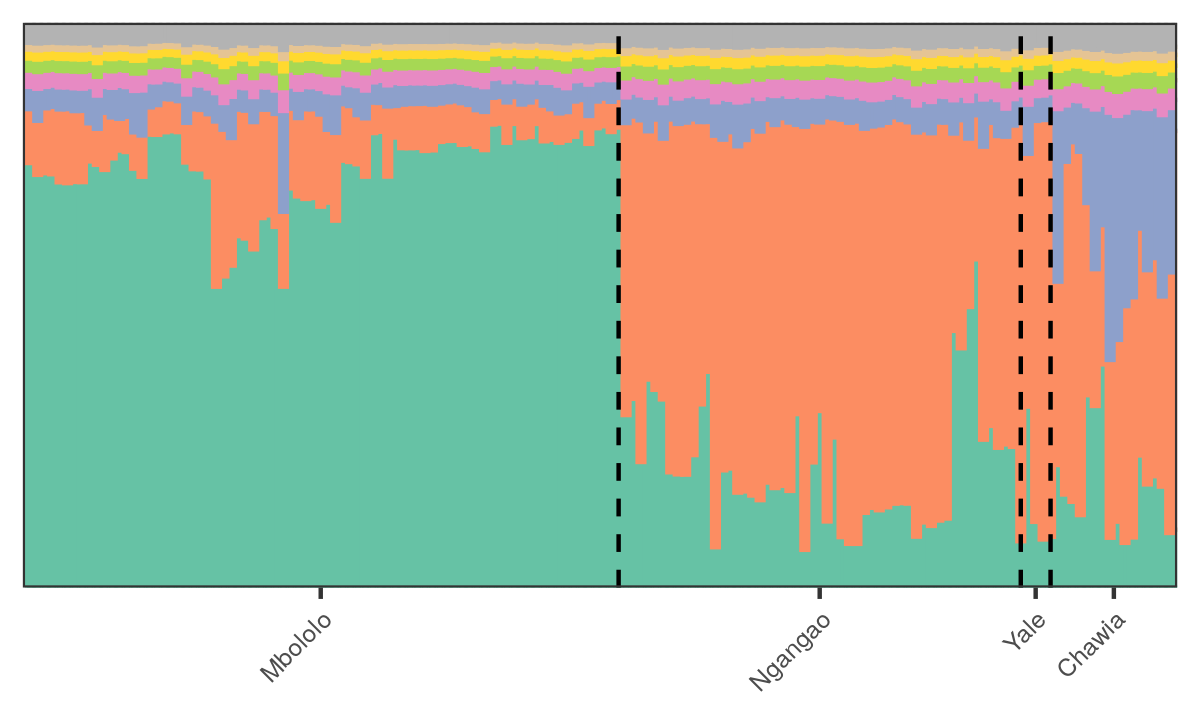
\includegraphics[width=0.980\linewidth,height=0.588\linewidth]{figure/stru_init_fit-1} 

}

\caption[The inferred individual admixtures at $\alpha_0 = 3$]{The inferred individual admixtures at $\alpha_0 = 3$. 
    Each vertical strip is an individual and each color
    a latent population.
    Lengths of colored segments represent the inferred admixture proportions.
    Individuals are ordered by the geographic region from which they were sampled
    (Mbololo, Ngangao, Yale, and Chawia).
    In the text, we refer to the green, orange, and purple latent populations 
    as population 1, 2, and 3, respectively. }\label{fig:stru_init_fit}
\end{figure}


\end{knitrout}


\subsubsection*{Sensitivity: number of populations}

We start by evaluating the sensitivity of the inferred number of populations
to the $\alpha$ parameter in the $\betadist{\nu_{nk}\vert 1, \alpha}$ stick distribution. 
Define the posterior quantity
\begin{align*}
\gpop(\eta; t)
&= \expect{\q(\z\vert\eta)}{\sum_{\k=1}^\kmax \ind{ 
\left(\sum_{\n=1}^{\nindiv}
\sum_{\l=1}^{\nloci}
\sum_{\i=1}^2
\z_{\n \l \i \k}\right) > \tau}},
\end{align*}
which is the expected number of populations in the data set that contains at least $\tau$ loci. 
We allow the option of setting $\tau > 0$ in order to count only the populations that comprise a non-negligible fraction of the data set. 


% 
% $\gpop$ counts a population as present if they contain at least $\tau$ loci. 
% When $\tau = 0$, $\gpop$ is equivalent to the expected in-sample number of clusters discussed in \secref{results_iris}, except the summation is now over individuals, loci, and chromosomes. 

At $\tau = 0$, $\gpop$ has a simple closed form expression as a function of the expectations of $\z_{\n \l \i \k}$; 
for $\tau > 0$, we resort to Monte Carlo estimates. 
Like the posterior quantity $\gclusterspred$ discussed in \secref{results_iris},
we use the re-parameterization trick to sample from $\q(\z\vert\eta)$. 
This allows us to condition on fixed draws from a distribution that is independent of $\eta$ (in this case, the underlying distribution is $\mathrm{Uniform}[0, 1]$); 
these fixed draws are shared across every computation of $\gpop(\eta; \tau)$ below. 

The expected number of latent populations is sensitive to $\alpha$ (\figref{stru_alpha_nclusters}).
Without any thresholding ($\tau = 0$),
the expected number of populations quickly increases as $\alpha$ increases; 
in fact, it nearly saturates at $\kmax = 20$ when $\alpha = 7$. 
This sensitivity is likely due to the fact that the non-thresholded quantity 
is highly dependent on the behavior of small, nearly unoccupied populations;
even though the probability of a single locus belonging to these rare populations is small, the probability that \textit{none} of the $\nindiv \times \nloci \times 2$ observed genotypes belong to these rare populations is non-negligible.  

This motivates the use of thresholding in reporting the number of populations. 
We consider two thresholds, $\tau = 20$ and $\tau = 40$,
corresponding to approximately 
$2\%$ and $4\%$ 
of the total number of loci in the data set, respectively. '
The thresholded estimates for the number of populations is stil
moderately sensitive to the value of $\alpha$. 
When refitting the variational approximation at $\alpha = 1, \ldots, 7$,
the thresholded quantities vary between two and four
latent populations. 

The linear approximation imperfectly captures the results observed by refitting. 
We formed the linear approximation at $\alpha_0 = 3$ and computed 
$\gpop$ using the linearly approximated variational parameters
$\etalin(\alpha)$ for $\alpha = 1, \ldots, 7$. 
For this range of $\alpha$, $\etalin(\alpha)$ and the refitted parameters 
$\etaopt(\alpha)$ almost perfectly agree on values of $\gpop$ with $\tau = 0$. 
However, when $\tau = 20$ and $\tau = 40$, 
the linearly approximated parameters 
underestimated the true sensitivity of $\gpop$ found by refitting. 
In particular, the linearly approximated parameters failed to produce
the reduction to two latent populations at $\alpha = 1$ observed in the refits.


\begin{knitrout}
\definecolor{shadecolor}{rgb}{0.969, 0.969, 0.969}\color{fgcolor}\begin{figure}[!h]

{\centering 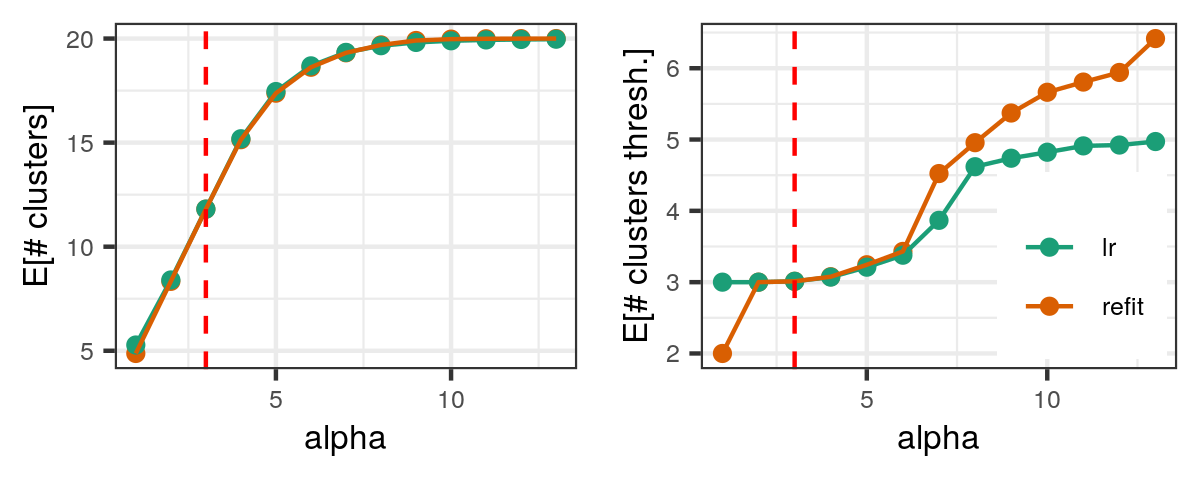
\includegraphics[width=0.980\linewidth,height=0.431\linewidth]{figure/stru_alpha_nclusters-1} 

}

\caption[The expected number of (thresholded) 
    populations in the thrush data as $\alpha$ varies.
    We computed the linear approximation at $\alpha_0 = 3$, and
    we compare the 
    results under the linearly approximated variational parameters with the
    results observed after refitting]{The expected number of (thresholded) 
    populations in the thrush data as $\alpha$ varies.
    We computed the linear approximation at $\alpha_0 = 3$, and
    we compare the 
    results under the linearly approximated variational parameters with the
    results observed after refitting. 
    Thresholds at $\tau = 20$ and $\tau = 40$ corresponding to 
    approximately 
    $2\%$ and $4\%$ 
    of the total number of loci in the data set, respectively. }\label{fig:stru_alpha_nclusters}
\end{figure}


\end{knitrout}

We provide some more intuition concerning the thresholded estimate for the number of populations.
Our posterior quantity $\gpop$ is closely related to the expected number of loci belonging to each population,
defined as
\begin{align*}
\gloci(\eta; k)
&= \expect{\q(\z\vert\eta)}{\sum_{n=1}^{\nindiv}
\sum_{l=1}^{\nloci}
\sum_{i=1}^2
\z_{\n l i \k}}. 
\end{align*}

\figref{stru_alpha_cluster_weights} plots $\gloci$ for the first six populations 
as $\alpha$ varies.
The expected number of loci at the initial fit, $\gloci(\etaopt(\alpha_0); k)$,
is at least 100 for populations $\k = 1, 2,$ and $3$ and 
less than 
12
for the remaining populations.  
A sample of memberships $\z\sim \q(\z\vert\etaopt(\alpha_0))$ will 
almost always have at least $\tau$ loci allocated to populations 1, 2, and 3, 
while the allocations to each remaining population will almost always be below $\tau$, for either $\tau = 20$ or $\tau = 40$. 
Thus, at $\alpha = \alpha_0$ there then are clearly 3 populations by our definition of $\gpop$, for either $\tau$.

At $\alpha = 7$, the expected number of loci belonging to population 4
increases to 
$20.7$, 
a new population emerges above the threshold at $\tau = 20$. 
Both the linearly approximated and the refitted variational parameters agree on this shift in allocation to population 4. 
On the other hand, under the refitted variational parameters at $\alpha = 1$, 
the expected number of loci belonging to population 3 decreases to 
$6.7$, 
below the thresholds $\tau = 20$ and $\tau = 40$. 
Thus, the expected number of latent populations with allocations above
either threshold decreases to two. 
The linearly approximated parameters
under-estimated this decrease in allocation to population 3, and 
therefore continued to estimate three latent populations even at $\alpha = 1$. 


\begin{knitrout}
\definecolor{shadecolor}{rgb}{0.969, 0.969, 0.969}\color{fgcolor}\begin{figure}[!h]

{\centering 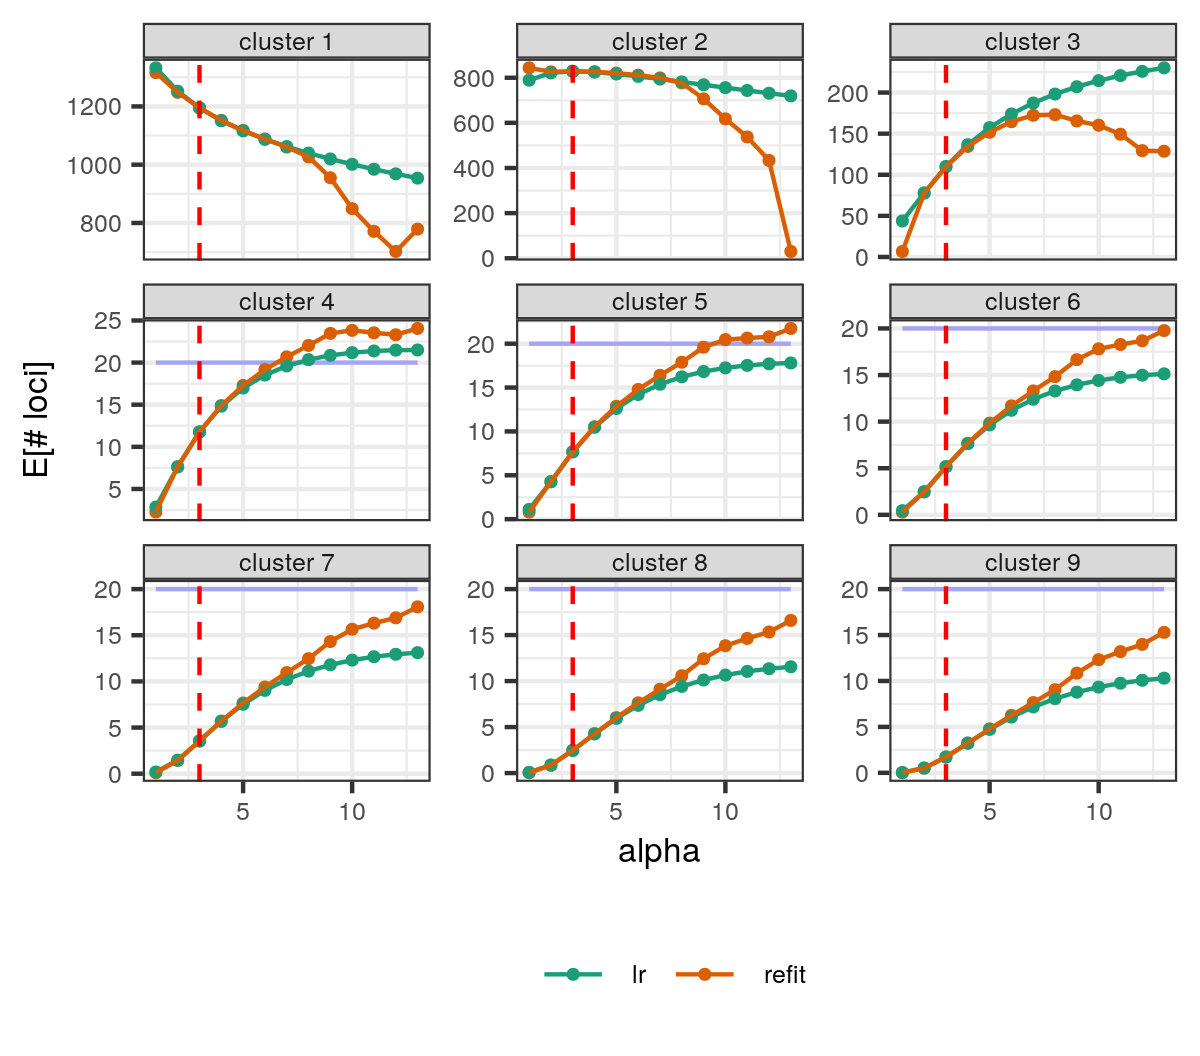
\includegraphics[width=0.980\linewidth,height=0.588\linewidth]{figure/stru_alpha_cluster_weights-1} 

}

\caption[The expected number of loci per population as $\alpha$ varies]{The expected number of loci per population as $\alpha$ varies. }\label{fig:stru_alpha_cluster_weights}
\end{figure}


\end{knitrout}

\subsubsection*{Sensitivity: individual admixtures}

Examining the inferred admixtures in \figref{stru_init_fit} provides clues into the historical migration patterns of the genotyped individuals. 
For example, while individuals collected from the Mbololo region are inferred to be admixed primarily with population 1, 
several individuals from this region have abnormally large admixture proportions of population 2. 
Conversely, while individuals collected from the Ngangao region are admixed primarily with population 2, a few of these individuals have abnormally large
admixture proportions of population 1. 
This suggests that some migration has occured between the Mbololo and Ngangao regions. 

We evaluate the sensitivity of this conclusion to possible prior perturbations. 
Consider the posterior statistic 
\begin{align*}
\gadmix(\eta; \mathcal{N}, k) = 
 \expect{\q(\pi\vert\eta)}{\frac{1}{|\mathcal{N}|}\sum_{n\in\mathcal{N}}
\pi_{\n\k}},
\end{align*}
the average admixture proportion of population $\k$ in a set of 
individuals $\mathcal{N}$. 

We present results on three variations of $\gadmix$: 
$\mathcal{N} = \{26, ..., 31\}$ and $k = 2$, 
corresponding to the six individuals from the Mbololo region with outlying proportions of population 2; 
$\mathcal{N} = \{125, ..., 128\}$ and $k = 1$, 
corresponding to the four individuals from the Ngangao region with outlying proportions of population 1; 
$\mathcal{N} = \{139, ..., 155\}$ and $k = 3$,
corresponding to all individuals from the Chawia region. 
In the last case, we are studying the sensitivity of haing a third latent
population present, a population which primarily appears in Chawia individuals. 

We construct the worst-case negative perturbation for each variant of $\gadmix$.
We consider the negative direction because we are interested in testing the 
robustness of these patterns' existence.
For each worst-case perturbation, we examine the effect on its respective 
posterior quantity $\gadmix$
as $t \rightarrow 1$ in 
the perturbed prior $\p(\nu\vert \t) = \p_0(\nuk)\exp(\t\phiworstcase(\nuk))$ (\figref{stru_func_sens}).
Under the linearly approximated variational parameters, 
the admixture proportion of population 2 in the outlying Mbololo individuals is nearly halved at $t = 1$. 
The same quantity computed after refitting the model 
confirms the sensitivity predicted by the linear approximation. 
On the other hand, the presence of population 1 in the outlying Ngangao individuals appears to be insensitive even after this worst-case perturbation. 
The linearly approximated and the refitted variational parameters again
agree on this conclusion. 
Finally, the presence of population 3 in the Chawia individuals is anticipated to be sensitive by the linear approximation, as this admixture proportion steadily decreases as $t\rightarrow 1$. 
However, under the refits, this admixture proportion does not decrease steadily but rather levels off after $t = 0.5$. 



\begin{knitrout}
\definecolor{shadecolor}{rgb}{0.969, 0.969, 0.969}\color{fgcolor}\begin{figure}[!h]

{\centering 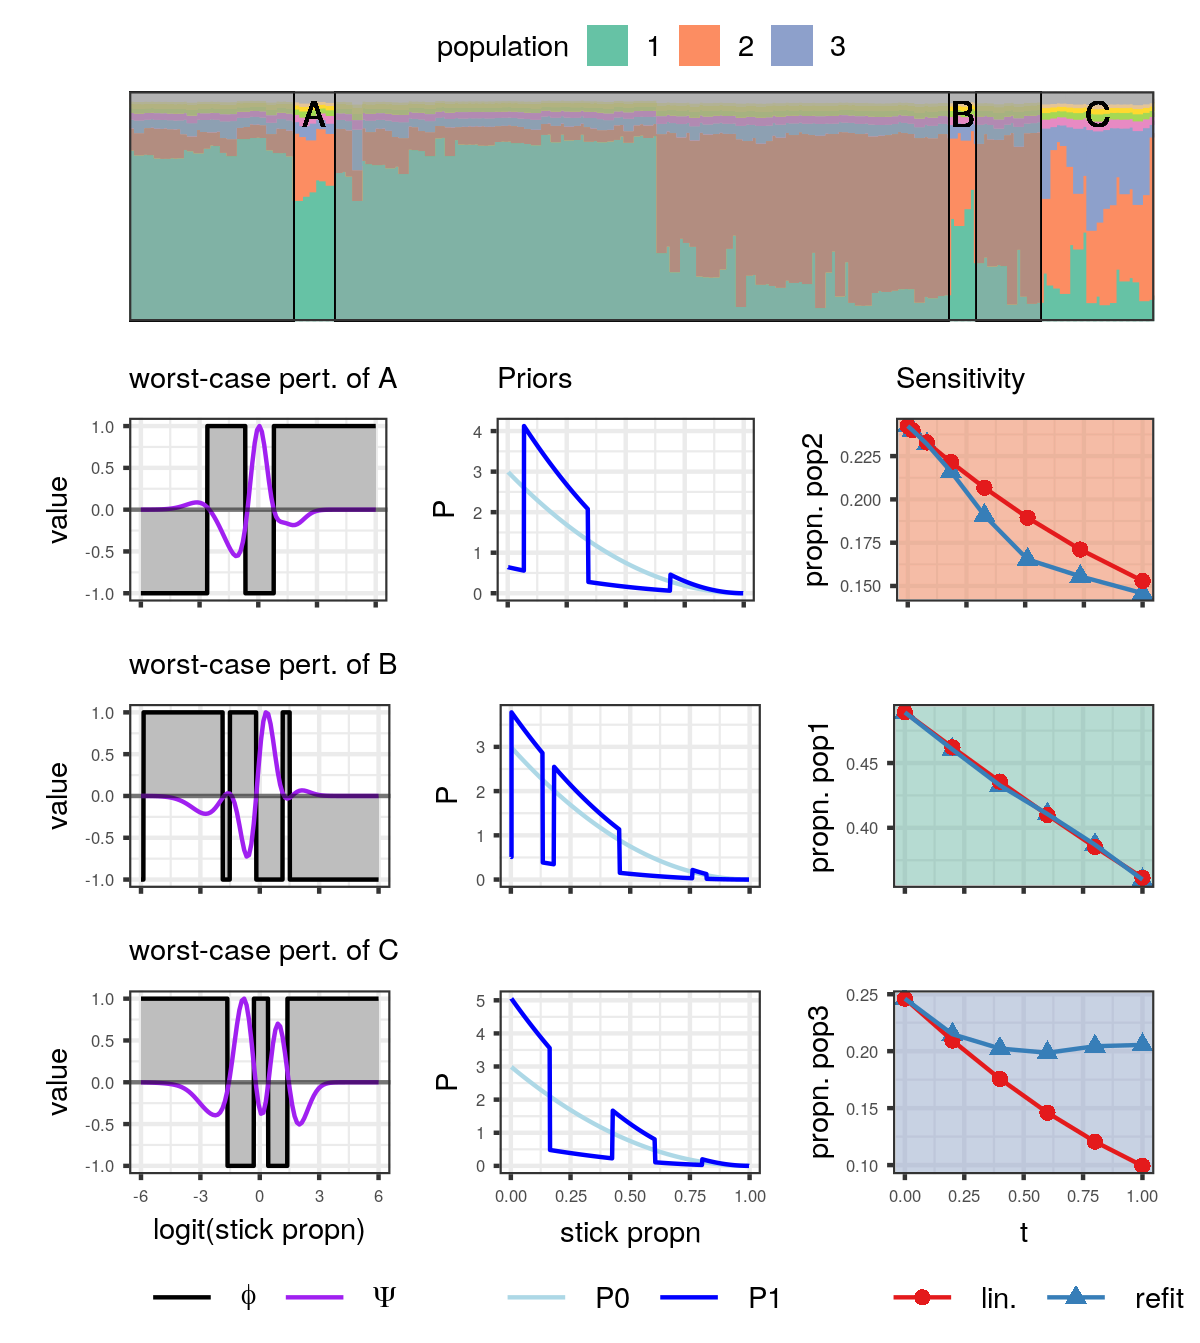
\includegraphics[width=0.980\linewidth,height=1.098\linewidth]{figure/stru_func_sens-1} 

}

\caption[Sensitivity of inferred admixtures for several outlying individuals]{Sensitivity of inferred admixtures for several outlying individuals. 
     For individuals A, 
     we examine the sensitivity of the admixture proportion of population 2.
     For individuals B, 
     we examine the population 1 admixture
     For the individuals C, we examine the population 3 admixture.
     (Left column) The worst-case negative perturbation with unit $L_\infty$-norm 
     in grey,
     plotted against the influence function in purple
     (scaled to also have $L_\infty$ norm equal to 1). 
    (Middle column) The effect of the perturbation on the prior density. 
    (Right column) Effects on the inferred admixture. }\label{fig:stru_func_sens}
\end{figure}


\end{knitrout}

discussion of overall findings

compute time. 

\begin{table}[tb]
\centering
\caption{Compute time of results on the structure dataset. }
\begin{tabular}{|r|r|}
\hline 
    & time (seconds) \\ 
    \hline 
    Initial fit & 7 \\
    \hline
    Hessian solve for $\alpha$ sensitivity & 
        0.32\\
    Linear approx. $\eta^{lin}(\alpha)$ for $\alpha = 1, ..., 10$ & 
        0.0059\\
    Refits $\eta(\alpha)$ for $\alpha = 1, ..., 10$ & 
        34\\
    \hline
    The influence function & 0.59\\
    Hessian solve for worst-case $\phi$ &
        0.38\\
    Linear approx. $\eta^{lin}(\epsilon)|_{\epsilon = 1}$ 
      for worst-case $\phi$ &
        0.00085\\
    Refit $\eta(\epsilon)|_{\epsilon = 1}$ 
      for worst-case $\phi$ &
        13\\
    \hline
\end{tabular}
\end{table}

\subsection{Limitations of local sensitivity}

In this final subsection, 
we discuss some examples where 
the linear approximation $\etalin(t)$ is a poor subsitute 
for $\etaopt(t)$.  
This occurs when $\etaopt(t)$ is highly nonlinear in $t$. 
The examples discussed below use the STRUCTURE model and 
dataset presented in the
subsection above, and 
we examine results after
the worst-case perturbation ``A" in \figref{stru_func_sens}.

Recall from \figref{stru_func_sens} that the linear approximation agreed with the refit in predicting the diminished admixture proportion of population 2 
in the outlying Mbololo individuals (individuals ``A")
at the perturbed prior $\p_1 = \p_0\exp(\phiworstcase)$. 
However, while the linear approximation was able to 
capture the change in overall admixture proportion, 
it does not perform uniformly well over all individuals 
(\figref{stru_func_sens_admix}). 
For example, the admixture proportion of population 2 in individual $n = 25$
dramatically increased after refitting with the perturbed prior $\p_1$. 
The linear approximation failed to detect this change. 


\begin{knitrout}
\definecolor{shadecolor}{rgb}{0.969, 0.969, 0.969}\color{fgcolor}\begin{figure}[!h]

{\centering 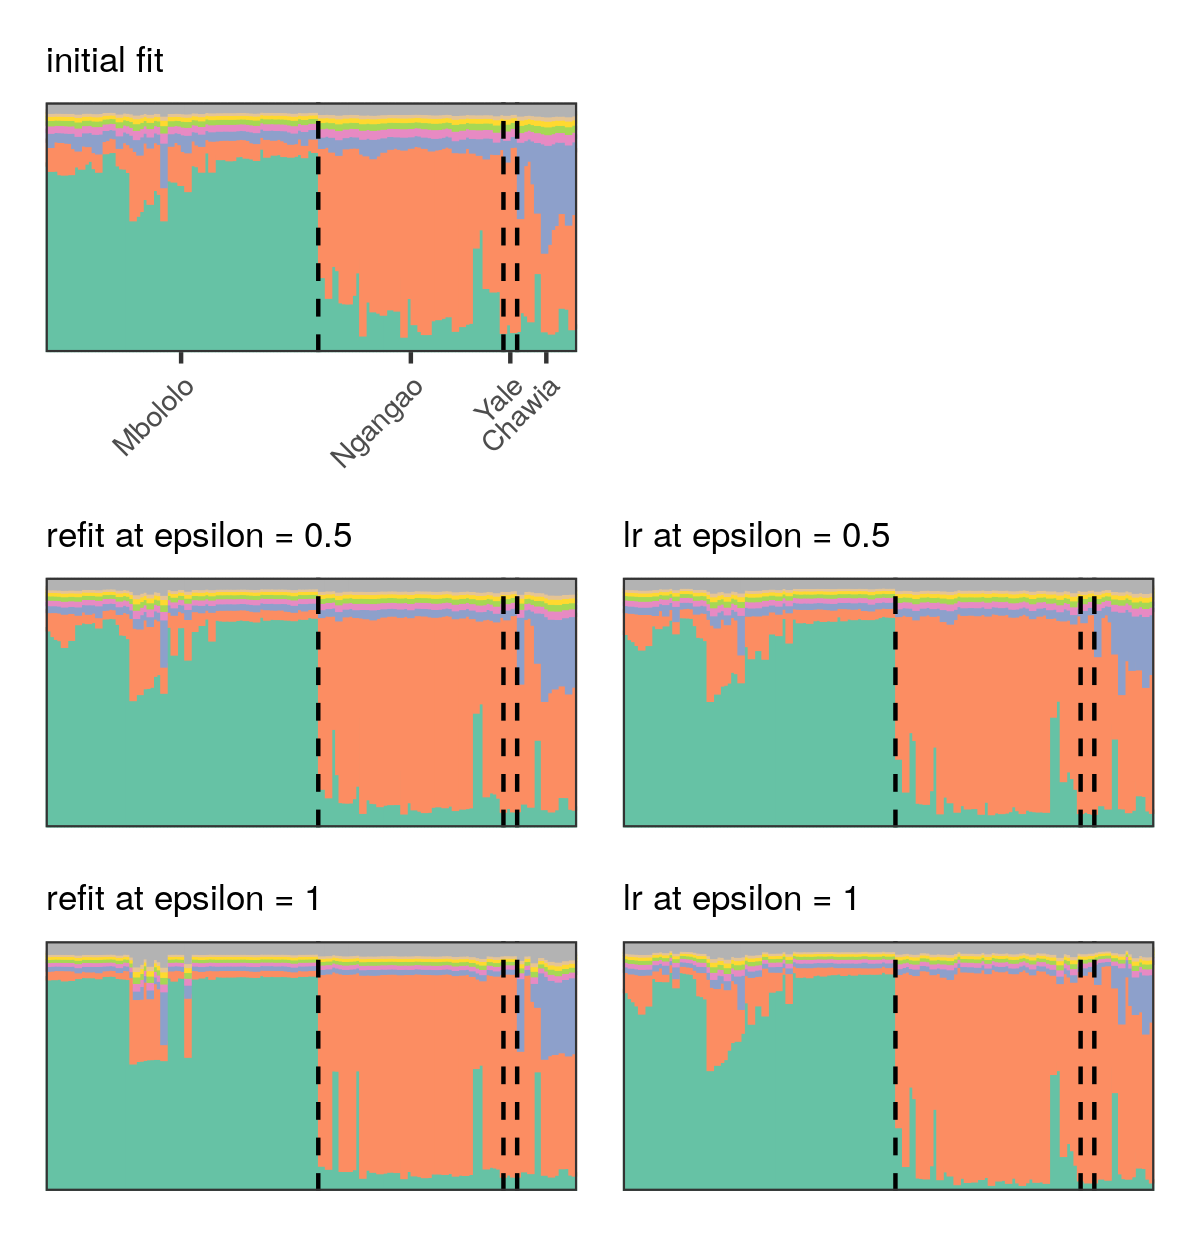
\includegraphics[width=0.980\linewidth,height=0.392\linewidth]{figure/stru_func_sens_admix-1} 

}

\caption{Inferred admixtures after the worst-case perturbation 
     to individuals ``A" (see Figure~\ref{fig:stru_func_sens} for perturbation). }\label{fig:stru_func_sens_admix}
\end{figure}


\end{knitrout}

\figref{stru_lin_bad_example} examines this individual ($n = 25$) more closely. 
The bottom row plots this individual's 
admixture proportions as $\t$ varies from 0 to 1 in the perturbed prior
$\p(\nu\vert \t) = \p_0(\nuk)\exp(\t\phiworstcase(\nuk))$. 
The linear approximation poorly captured the change in admixture proportions observed after refitting, particularly for values of $\t$ close to 1. 
Even though our linear approximation retains non-linearities in the mapping from variational parameters to the posterior statistic,
for this perturbation, the mapping from prior parameter
$\t$ to the relevant variational parameters
is highly non-linear. 
This latter mapping is what we linearize, and thus what causes our approximation to fail in this case. 
Specifically, the location parameter of the variational distribution 
on the logit stick-breaking proportions (which recall are Gaussian)
is concave for the first stick-breaking proportion -- the location parameter increases for small $\t$ at first, then decreases. 
Our approximation assumes a linear relationship between the location parameter and $\t$. 
Therefore, the corresponding admixture mixture proportion of population 1 is mis-estimated by the linear approximation. 
Furthermore, because our linearized variational parameter over-estimated the length of the first stick, 
and the second admixture proportion being a product of the remaining stick times the second stick-breaking proportion, 
the linearized variational parameters then under-estimates the admixture proportion of population 2. 




\begin{knitrout}
\definecolor{shadecolor}{rgb}{0.969, 0.969, 0.969}\color{fgcolor}\begin{figure}[!h]

{\centering 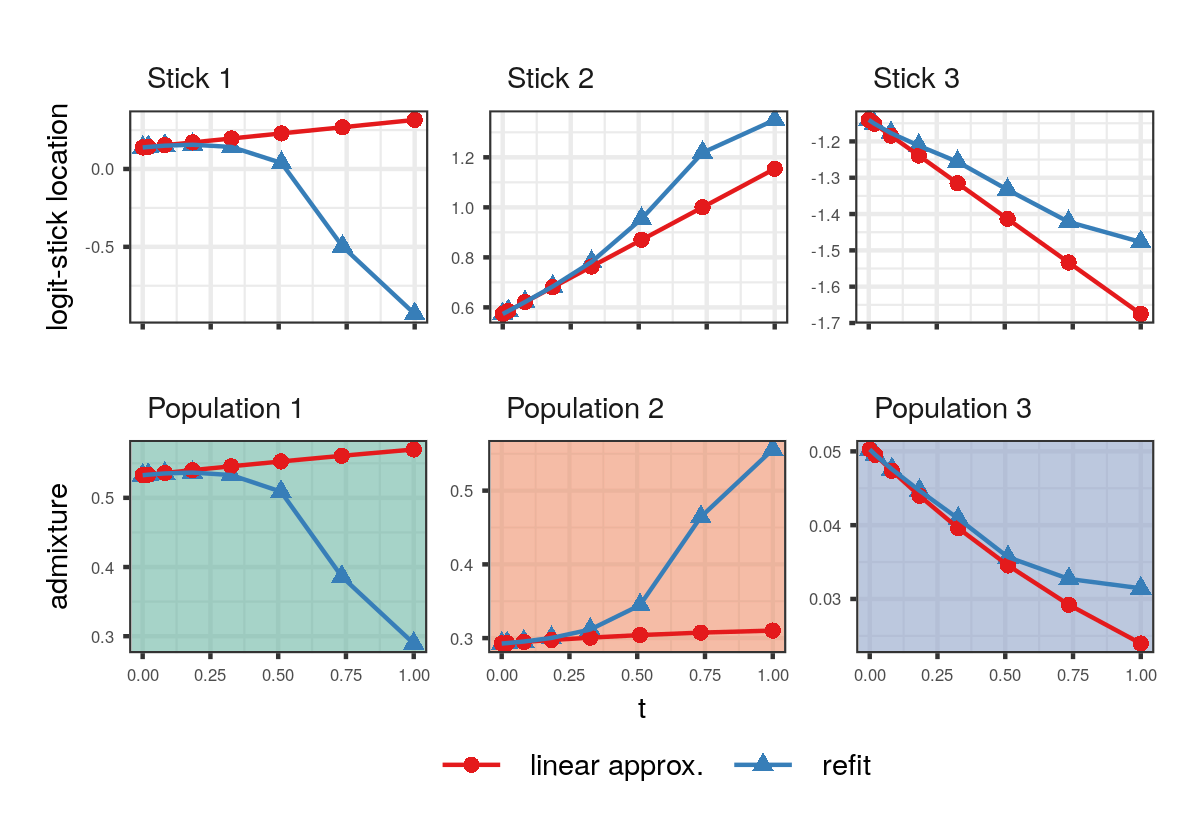
\includegraphics[width=0.980\linewidth,height=0.666\linewidth]{figure/stru_lin_bad_example-1} 

}

\caption[An individual $(\n = 26)$ for which 
    the linearly approximated variational parameters
    poorly captured the 
    change in admixture observed after refitting
    as $\t \rightarrow 1$]{An individual $(\n = 26)$ for which 
    the linearly approximated variational parameters
    poorly captured the 
    change in admixture observed after refitting
    as $\t \rightarrow 1$. 
    (Top row) the change in location parameter of the normally
    distributed logit-sticks, for the first three sticks. 
    The response here is a variational parameter, so 
    the approximation (red) is necessarily linear with respect to $\t$. 
    (Bottom row) the change in the inferred admixtures for 
    populations 1, 2, and 3. }\label{fig:stru_lin_bad_example}
\end{figure}


\end{knitrout}



\figref{stru_fully_lin_example} shows a similar situation for individual $n = 74$. 
The linearized variational parameters grossly over-estimated the length of the first stick,
resulting in the later admixture proportions being under-estimated. 
The third admixture proportion was particularly poorly approximated by the linearized variational parameters. 
Given the recursive nature of the relationship between admixtures and stick-breaking proportions, errors at early sticks affect later admixture proportions. 
Fully linearizing the mapping from $\t$ to $\g(t)$ and forming the approximation 
$\glin(t)$ (\eqref{}) avoids this problem. 
In this example, $\glin(t)$ outperforms $\g(\etalin(t))$, where $\g$ is the admixture proportion of population 3. 
In all the previous examples (including the example in \figref{stru_lin_bad_example}), 
computing $\g(\etalin(t))$, and thus retaining the non-linearities in the mapping from $\eta\mapsto \g$,
does no worse, and is usually better,
than the fully linearized version, $\glin(\t)$---as can be seen by drawing tangent lines of the refitted curve at
$\alpha = \alpha_0$ or $t = 0$
for 
\figref{iris_alpha_sens,
stru_alpha_nclusters, 
stru_alpha_cluster_weights, 
stru_lin_bad_example}. 
It is likely that $\g(\etalin(t))$ outperforms $\glin(\t)$ for most posterior quantities, though as we see in \figref{stru_fully_lin_example},
this is not guaranteed to always be true.  


% In the examples above, we only linearized the mapping $\epsilon \mapsto \etaopt(\epsilon)$. 
% In most examples, we find that retaining the non-linearities from $\eta\mapsto g$ performed as well, or better than, fully linearizing the mapping from $\epsilon \mapsto \eta$. 
% There are exceptions, as we discuss below. 


\begin{knitrout}
\definecolor{shadecolor}{rgb}{0.969, 0.969, 0.969}\color{fgcolor}\begin{figure}[!h]

{\centering 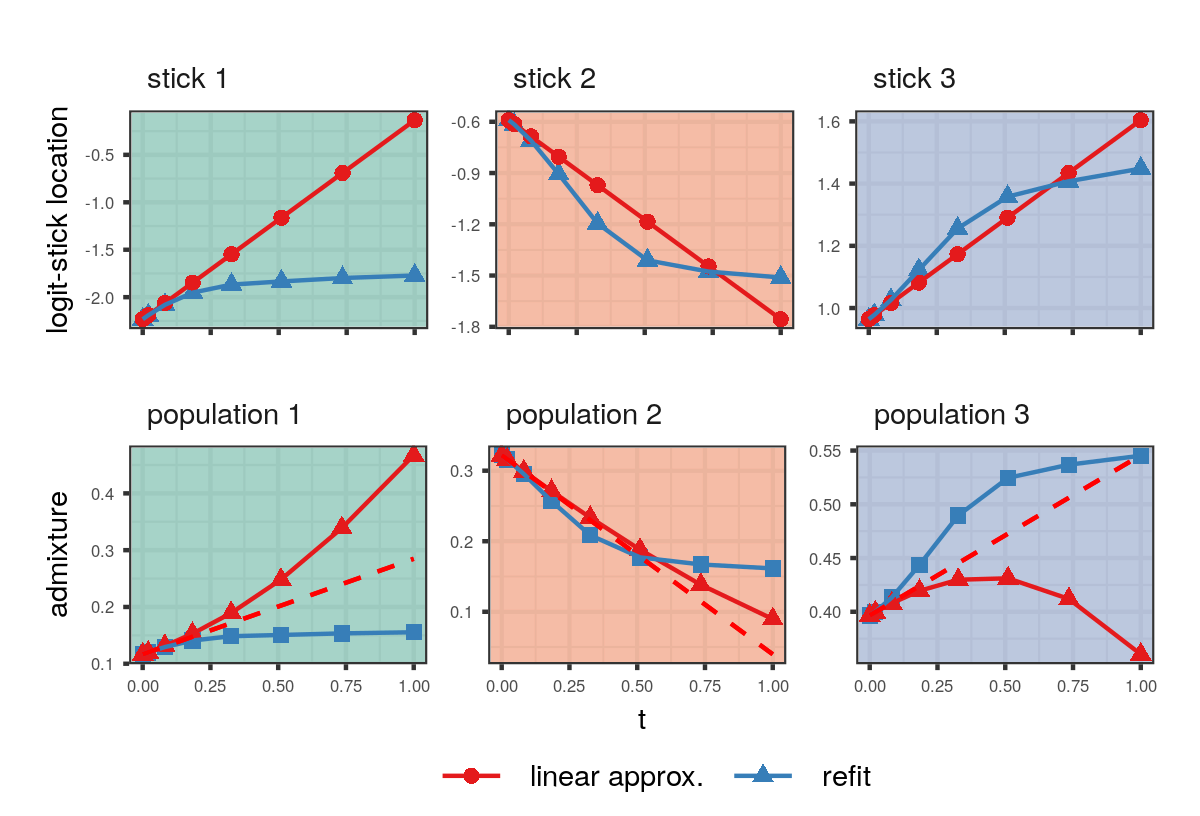
\includegraphics[width=0.980\linewidth,height=0.666\linewidth]{figure/stru_fully_lin_example-1} 

}

\caption[An example where 
    linearizing the posterior quantity itself outperforms 
    linearizing the variational parameters only]{An example where 
    linearizing the posterior quantity itself outperforms 
    linearizing the variational parameters only. 
    Shown are logit-stick location parameters (top row) and
    inferred admixtures (bottom row)
    for individual $n = 74$ and populations $k = 1, 2$ and $3$. 
    In dashed red is the approximation formed by linearizing the
    inferred admixture $\mathbb{E}_{\q}[\pi_{\n\k}]$ with respect to prior
    parameter $t$.
    On the admixture proportion of population 3, 
    this approximation outperforms linearizing the variational parameters only. }\label{fig:stru_fully_lin_example}
\end{figure}


\end{knitrout}



